\def\todoNextRevision#1{{\color{blue}[[``todo next revision'': #1]]}}

\chapter{Agent-Based Traffic Assignment \who{Nagel}}
\label{ch:abta}
% ##################################################################################################################

\hfill \textbf{Authors:} Kai Nagel, Gunnar Flötteröd

\begin{center} 
\includegraphics[width=0.25\textwidth, angle=0]{frontmatter/figures/MATSimBook.jpg} \end{center}

%%%%%%%%%%%%%%%%%%%%%%%%%%%%%%%%%%%%%%%%%%%%
%%%%%%%%%%%%%%%%%%%%%%%%%%%%%%%%%%%%%%%%%%%%
\kai{Anfrage an Verlag, sobald wir mal Zeit haben.}

% ##################################################################################################################

%\ah{Gunnars Relaxation-Mail, 26.11.}
%\kai{what is this???}

%##################################################################################################################


\section{Introduction}
\label{sec:agenbased-dta-intro}

This chapter presents MATSim from a dynamic traffic assignment (DTA) perspective. 
The following material is an abridged and edited version of \citet{NagelFloetteroed2009IatbrResourceInBook}.

\kai{how much of this introductions should stay?  Intuitively, we should justify matsim elsewhere.}

\gunnar{Ich habe jetzt erstmal ziemlich viel auskommentiert.}

% Despite of the substantial progress made in activity-based demand modeling and computational simulation techniques, many dynamic traffic assignment (DTA) models suffer from simplified behavioral representations. Two major issues are:
% \begin{enumerate}
% \item Consistently incorporated choice dimensions rarely go beyond route choice.
% \item Decision protocols rarely go beyond stochastic equilbrium models.
% \end{enumerate}

%%Either item can be explained both from a modeling perspective and a
%%computational perspective. 
%
% M.E. ist führt "introduction" derzeit induktiv auf diesen Punkt hin.
% Sehe nicht, wieso es hilfreich ist, dies auch deduktiv zu erwähnen. Kai

%%However, this requires some preliminary notes on the notion of
%%``network dynamics''.
%
% Denke, dies war eine Ankündigung des Abschnittes über
% "doubly-dynamic assignment et al".  Habe den jetzt aber (erstmal?)
% nach "within-day replanning" verschoben, weil ich gar nicht sehe,
% wieso er hier benötigt wird (trotz der Behauptung, dass er nötig
% wäre).  Kai


%%\subsection{Behavioral modeling challenges in dynamic traffic assignment}

%%\mnote{add choice dimensions}

% Most DTA models take time-dependent origin/destination (OD) matrices 
% as inputs and equilibrate time-dependent route flows \citep{peeta-2001}.
% In this, they ignore the feedback of changing network conditions on
% higher--level choice dimensions such as departure time choice, mode
% choice, activity schedule choice, and such. It appears natural to
% extend the feedback to all choice dimensions, which also requires to
% consistently account for them at the assignment level.

%%\mnote{take care of constraints}

% One essential aspect of introducing more behavior into DTA
% models is to account for the dynamic constraints subject
% to which real travelers make their decisions: For example,
% going somewhere by car is likely to imply that later travel is done by
% car as well, or going shopping during a lunch break renders later
% shopping trips unnecessary.  However, as long as the demand
% representation is in terms of temporally at most loosely coupled OD
% matrices, it discards much of the structure of real travel decisions.

%%\todoKai{Hier koennte die "uebliche" Kritik an der Kopplung ABDG 
%%-- assignment ueber OD Matrizen gut passen. Gunnar}
%
%Vielleicht reicht das, was da jetzt steht. Kai

%%\subsection{Behavioral simulation challenges in dynamic traffic assignment}
%\subsection{Introducing (more) behavior into assignment models}

%%\mnote{intractable number of commodities in macroscopic models}
%mathematical reformulation possible by increasing number of
%  commodities accordingly; computationally intractable}

% Having said this, the question arises how to implement and simulate a
% demand model that properly accounts for general choice dimensions and
% constraints. A specification in terms of analytical equations exhibits
% desirable formal properties and enables the application of sound
% mathematical solution procedures \citep[see,
%   e.g., the supernetworks approach in][]{sheffi-1985,NagurneyEtcSupernetworks}. However, if the
% structure of the behavioral model is to be properly accounted for, the
% dimension of the problem to be solved increases
% vastly. Mathematically, this can be accounted for by increasing the
% number of commodities in the macroscopic model, which accounts for the
% likewise increased degree of heterogeneity in the population that is
% naturally revealed if the demand model becomes more detailed. However,
% because of the combinatorial nature of all possible choices a traveler
% faces during a single day, the number of commodities quickly becomes
% computationally intractable.

%%\mnote{usim as behavior vs.\ usim as MC technique}

% At this point, microsimulation naturally enters the picture. Observing
% that the solution of a DTA model that comprises a large number of
% commodities is in fact 
% %
% a choice distribution over all of these commodities, rather than
% %
% a vector of deterministic expectation values,
% %
% Monte Carlo techniques for the realization of this distribution come
% to mind. Assuming without loss of generality the most disaggregate
% case where every single traveler constitutes one commodity, the
% micro-simulation of individual travel behavior can be re-interpreted
% as a Monte Carlo technique to draw from the underlying distributions.
% That is, while the microsimulation of individual behavior has
% an intuitive meaning, it maintains a mathematically consistent
% interpretation.

%%\mnote{use MC techniques similarly in random coefficient RUM}

%%\todoKai{Need to check this paragraph. Is by now probably redundant with
%%the footnote in Section "Behavioral calibration". Gunnar}
%
%Von mir aus können wir es (auch) hier lassen, als weiteres Beispiel,
%wie dann MC Simulation genommen wird. Kai

% The transition from multi-commodity flows to microsimulation faces a
% symmetrical development in the field of random utility modeling:
% The classical multinomial logit model allows to estimate different
% coefficients for different segments of the population of decision
% makers, but the granularity of this segmentation is limited 
% \citep{ben-akiva-1985}. Random coefficient models overcome this
% confinement in that they allow for a whole distribution of
% behavioral parameters. However, since random coeffient models have
% difficult mathematical forms, their evaluation and estimation is
% conducted based on Monte Carlo simulation \citep{train-2003}.

%%\mnote{balance between computational efficiency and modeling}

% Even the micro-simulation approach comes with a substantial
% computational burden. The simulation of millions of individual travelers
% on a detailed network requires a careful balance between modeling precision
% and computational efficiency, and it requires to incorporate substantial
% computer science and software design knowledge in order to implement
% operational simulation systems. By now, most of the computational problems 
% can be considered to be solved at least at a basic level
% of modeling sophistication even for large-scale scenarios, and the most
% critical research question has become to move these solutions into
% a more consistent modeling framework while maintaining their favorable
% computational properties.

%%\subsection{This paper}

% This chapter starts in Section~\ref{sec:equil-models-day} with a discussion
% of how the iterative solution procedure of congested assignment models
% can be re-interpreted as a behavioral learning loop.  This includes,
% as important elements, the move from continuous traffic streams to
% discrete individual travellers, and the inclusion of additional choice
% dimensions beyond route choice.  

% Section~\ref{sec:agent-based-simul} then concentrates on how these
% concepts can be implemented in a microscopic, behaviorally-oriented
% (``agent-based'') simulation.  Most of the text concentrates on what
% we call \emph{agent-based stochastic user equilibrium (SUE)};
% here, the SUE formulation is traced
% back to its origins in that the simulated travelers are assumed to
% have a choice set consisting of several alternatives, and that, in
% every iteration, they make a deliberate, probabilistic choice from
% this set.  It is noted that this has useful parallels with
% co-evolutionary computation, and in consequence algorithms and methods
% from that area can be used to address the agent-based SUE problem.

%% A regular challenge with agent-based simulations is how to set the
%% microscopic rules such that the macroscopic outcome (sometimes called
%% ``emergence'') corresponds to known or desired behavior.
%% Section~\ref{sec:Calibration} demonstrates how this challenge can be
%% addressed in the area of behavioral traffic simulation.
% --- or, in
%fact, in any area where the behavior is based on models
%that make randomized choices between discrete alternatives.

%%All developments in this chapter assume within-day dynamic behavior,
%%i.e.\ a development of the traffic and behavioral patterns along the
%%time-of-day axis.  The typical equilibrium interpretation will,
%%however, assume that there is no within-day \emph{replanning}.  Since
%%this is clearly an important behavioral dimension,
%%Section~\ref{sec:with-day-repl} will investigate some of its consequences.  
%---
%The chapter finishes with a conclusion in Section~\ref{sec:conclusion}.






%%\vfill\eject
%%%%%%%%%%%%%%%%%%%%%%%%%%%%%%%%%%%%%%%%%%%%
%%%%%%%%%%%%%%%%%%%%%%%%%%%%%%%%%%%%%%%%%%%%
%\section{Equilibrium models and day-to-day replanning}
%\label{sec:equil-models-day}

The traffic assignment problem, no matter if macroscopic or
microscopic, static or dynamic, trip-based or agent-based, is to
identify a situation in which travel demand and travel supply (network
conditions) are consistent with each other. The travel demand results
from a demand model that reacts to the conditions in the network, and
the network conditions are the output of a supply model
(network loading model) that takes travel demand as its input. That
is, a solution of the traffic assignment problem describes an 
equilibrium between travel demand and travel supply.

The arguably most intuitive mathematical formulation of this problem is 
in terms of a fixed point: Find a demand pattern that generates network 
conditions that in turn cause the same demand pattern to re-appear. This 
formulation is operationally important because it motivates a straightforward 
way of calculating an equilbrium by alternately evaluating the demand 
model and the supply model. If these iterations stabilize then a fixed 
point is attained that solves the traffic assignment problem.

The remainder of this chapter casts MATSim into this DTA framework.
Section~\ref{sec:agent-based-DTA-from-routes-to-agents} starts out from the
static and macroscopic route flow assignment and incrementally enriches this 
formulation into a dynamic and fully disaggregate agent-based assignment problem.
Section~\ref{sec:agent-based-simul} then turns to the problem of how to
simulate (solve) this model system, with a particular focus on MATSim's
coevolutionary approach. Section~\ref{sec:agentbased-dta-conclusion} concludes
the presentation.


\section{\label{sec:agent-based-DTA-from-routes-to-agents}From route swapping to agent plan choice}

In the following, an increasingly comprehensive specification of the traffic 
assignment problem is given that starts from the classical static user 
equilibrium model and ends with a fully dynamic model that captures 
arbitrary travel demand dimensions at the individual level. Computationally, 
the iterative fixed point solution procedure is carried throughout the 
entire development. Not by chance, this solution method also has a behavioral 
interpretation as a model of day-to-day replanning; see also Chapter~\note{REF: research avenues}.

We start by considering route assignment only. The generalization towards further 
choice dimensions will turn out to be a natural generalization of the route assignment problem.

\subsection{\label{static-macro-assignment}Static traffic assignment}

Consider a network of nodes and links, where some or all of the nodes are demand origins, 
denoted by $o$, and/or demand destinations, denoted by $d$. 
The constant demand $q^{od}$ in origin/destination (OD) relation $od$ splits up among a set of routes $K^{od}$. 
Denote the flow on route $k\in K^{od}$ by $r^{od}_k$, where $\sum_{k\in K^{od}} r^{od}_k = q^{od}$.

Most route assignment models either specify a User (Nash, Wardrop) equilibrium (UE) 
or a stochastic user equilbrium (SUE).  
A UE postulates that $r^{od}_k$ is zero for every route $k$ of non-minimal cost \citep{Wardrop1952TheoreticalAspects}:
\begin{eqnarray}
c(k)=\min_{s\in K^{od}}c(s) & \Rightarrow & r^{od}_{k}\geq0\\
c(k)>\min_{s\in K^{od}}c(s) & \Rightarrow & r^{od}_{k}=0
\end{eqnarray}
where $c(k)$ is the cost (typically delay) on route $k$.
 
An alternative, often-used approach is to distribute the demand onto
the routes such that a SUE is
achieved where users have different perceptions of route cost and
every user takes the route of \emph{perceived} minimal cost \citep{daganzo-1977}.
Mathematically, this means that the route flows fulfill some distribution
\begin{equation}
r^{od}_k = P^{od}_k(c(x(\{r^{od}_k\}))) \cdot q^{od}
\label{stoch-equil}
\end{equation}
where the route splits $P^{od}_k$ are a function of the network costs
$c(x)$, which depend on the network conditions $x$,
which in turn depend on all route flows $\{r^{od}_k\}$.

In either case, the model needs to be solved iteratively, 
which typically involves the following steps \citep{sheffi-1985}:

\begin{algorithm}[H]
\label{static-macro-routes}

\caption{Macroscopic and static route assignment}

\begin{enumerate}

\item \textbf{Initial conditions:} Compute some initial routes
  (e.g., best path on empty network for every OD pair).

\item \textbf{Iterations:} Repeat the following many times.

\begin{enumerate}

\item \textbf{Network loading:} Load the demand on the network along
  its routes and obtain network delays (congestion).

\item \textbf{Choice set generation:} Compute new routes based on the
  network delays.

\item \textbf{Choice:} Distribute the demand between the routes based
  on the network delays.

\end{enumerate} %\item \textbf{Iterations:} Goto 2.

\end{enumerate}

\end{algorithm}

Considering the network loading to be more on the ``physical'' side of the system, 
the behaviorally relevant steps are choice set generation and choice \citep{bowman-1998}.

\textbf{Choice set generation:} Often, the new routes are best paths
based on the last iteration (``best reply'' choice set generation).
The routes are generated within the iterations because an a priori
enumeration of all possible routes is computationally infeasible.

\textbf{Choice:} Usually, demand is shifted among the routes in a way
that improves consistency with the route choice model, assuming
in the simplest case
constant network delays: In a UE, the flow on the currently best routes
is increased at the cost of the other route flows (``best reply''
choice), whereas for a SUE the flows are shifted towards the desired
route choice distribution \citep[often a version of multinomial logit,
  e.g.,][]{dial-1971, cascetta-1996, ben-akiva-1999}. For
stability reasons, this shift is typically realized in some gradual
way that dampens the dynamics of the iterations. See below for more
discussion on convergence issues. 

The \textbf{iterations} are repeated until some stopping criterion is
fulfilled that indicates that a fixed point is attained.
%Optimally, the iterations reach a fixed point. 
In the best reply situation, the fixed point implies that no shift
between routes takes place, i.e., what comes out as the best reply to
the previous iteration is either the same or at least of the same
performance as what was used in the previous iteration.
Since in this situation no OD pair can unilaterally improve
by switching routes, this means that the system is at a Nash
equilbrium \citep[e.g.,][]{HofbSigmBook}.
In the SUE situation, the fixed point means that a route flow pattern 
$\{r^{od}_k\}$ is found that leads to exactly those network conditions the
travelers (the OD flows) perceived when choosing their routes,
giving nobody an incentive to re-route.

Behavioral dimensions beyond route choice that can be captured by a
static model are destination choice and elasticity in the
demand. However, no technical generality is lost when discussing only
route choice because both additional choice dimensions can be
rephrased as generalized routing problems on an extended network
\citep[``supernetwork''; see, e.g.,][]{sheffi-1985,NagurneyEtcSupernetworks}. 
%% \todoKai{Ich meine mich
%%  zu erinnern, dass das in dem Buch auftaucht. Habe es aber leider
%%  nicht in Reichweite... Gunnar}


\subsection{Dynamic traffic assignment}

As is well known, the above also works for \emph{dynamic} traffic
assignment \citep[DTA; see][]{peeta-2001}, where both the demand and the 
network conditions are now time-dependent and the time-dependent travel 
times in the network now define a physically meaningful progression of 
a demand unit through the network. 

The structure of the algorithm does not change. The individual steps now look as follows:
\begin{algorithm}[H]
\label{dynamic-macro-routes}

\caption{Macroscopic and dynamic route assignment}

\begin{enumerate}

\item \textbf{Initial conditions:} Compute some initial routing (e.g., best path on empty network
  for every OD pair and departure time).

\item \textbf{Iterations:} Repeat the following many times.

\begin{enumerate}

\item \textbf{Network loading:} Load all demand items on the network
  according to their departure times, let them follow their
  routes, and obtain network delays (congestion).

\item \textbf{Choice set generation:} Compute new routes based on the
  network delays.

\item \textbf{Choice:} Distribute the demand between the routes based
  on the network delays.

\end{enumerate} % \item \textbf{Iterations:} Goto 2.

\end{enumerate}

\end{algorithm}

Once more, \emph{if} the new routes are best replies (i.e., best paths
based on the last iteration), \emph{if} demand is shifted towards
these new routes, and \emph{if} these iterations reach a fixed point,
then this is a dynamic UE since the best reply dynamics means that no
traveler (no OD flow) can unilaterally deviate to a better route.  The
SUE interpretation carries over in a similar way.

Destination choice and elasticity in the demand apply naturally to 
the dynamic case as well. Beyond this, the dynamic setting also enables 
the modeling of departure time choice. Again, the sole consideration 
of route choice does at least technically not constitute a limitation 
because departure time choice can be translated into route choice in a 
time-expanded version of the original network \citep{vanderzijpp-2001}.


\subsection{Individual travelers}
\label{sec:indiv-trav}

Both in the static and in the dynamic case, it is possible to
re-interpret the algorithm in terms of individual travelers.  
%
In the static case, for every OD pair one needs to
assume a steady ($=$ constant) flow of travelers that enter the
network at the origin at a constant rate, corresponding to that OD flow.
A solution to the static assignment problem corresponds to the
distribution of the different travelers onto possibly different paths.

In the dynamic case, one needs to generate the appropriate number of
travelers for every OD pair and every time slot, and distribute them
across the time slot.  From then on, the triple (origin, destination,
departure time) is fixed for every simulated traveler, and its goal is
to find an appropriate path.  
%
%%\yyyy{"The variable $r_k^n$ will denote the route if the $n$th traveller uses the $k$th route." -- I moved this where it is used first (subsection on particle SUE). Gunnar}
%ok. kai
%
Arguably, in the dynamic case this re-interpretation is behaviorally
more plausible.

In a trip-based context, there are two major motivations to go from 
continuous flows to individual travelers:
\begin{itemize}

\item Traffic flow dynamics in complex network infrastructures are 
difficult to model in terms of continous flows 
\citep[e.g.,][]{floetteroed-2011a} but are relatively straightforward 
to simulate at the level of individual vehicles
\citep[][]{aimsun-www,mitsim-www,paramics-www,vissim-www}. 
Disaggregating an OD matrix into individual trip-makers allows to 
assign one vehicle to every trip-maker in the microscopic traffic flow 
simulation.

\item It is computationally inefficient to capture demand heterogeneity 
through a large number of commodity flows, whereas the sampling of 
trip-makers with different characteristics is fairly straightforward. 
For example, every vehicle can be given an individual route to its individual 
destination.

\end{itemize}

%%\todoKai{Ab hier verstehe ich den Absatz nicht mehr. Gunnar} This is
%%probably somewhat more obvious in the dynamic variant, where plausibly
%%every traveler should have her/his own departure time, in other
%%words, where the fiction of traffic ``streams'' can only be upheld
%%when time remains sufficiently aggregated (e.g.\ into hourly time
%%bins).

%%Note that ``assignment with individual travelers'' is really quite
%%similar to conventional assignment, except that it now has a
%%behavioral interpretation.  The disadvantage is that, in this new
%%person-based interpretation, one is bound to integer travelers,
%%implying on the one hand that one cannot have fractional flows, and on
%%the other hand that one needs to perform a network loading with that
%%many individual travelers, often millions (but see below
%%\todoKai{check}).  In some sense, the person-based approach works because
%%the number of travelers is large enough such that it approximates
%%continuous numbers.  On the other hand, in some sense this is also the
%%reason why the conventional assignment method was valid at all.
%
%Habe den Eindruck, dass obiger Absatz nicht mehr nötig ist.  25oct09, kai

For a finite population of heterogenous travelers, every single
traveler constitutes an integer commodity, and the \textbf{choice}
step hence needs to be changed from "gradually shift the route flows
towards something that is consistent with the behavioral model" into
"for a \emph{fraction} of travelers, assign a \emph{single}
behaviorally plausible route to each of these travelers". The gradual shift that
helps to stabilize the iterations in the continuous assignment carries
over here to an equally stabilizing "inert shift" in that not all travelers
change their routes at once. This is a consistent reformulation: If
one reduces the traveler size to $\varepsilon \rightarrow 0$ and
increases the number of travelers by a factor of $1/\varepsilon$,
a 10\% chance of
changing routes in the disaggregate case carries over to shifting 10\%
of all flows to new routes in the aggregate case (``\textbf{continuous
limit}'').

Apart from this, the iterations do not look much different from what
has been said before:

\begin{algorithm}[H]
\label{dynamic-micro-routes}

\caption{Microscopic and dynamic route assignment}

\begin{enumerate}

\item \textbf{Initial conditions:} Compute some initial routing (e.g., best path on empty network
  for every traveler).

\item \textbf{Iterations:} Repeat the following many times.

\begin{enumerate}

\item \textbf{Network loading:} Load all travelers on the network
  according to their departure times, let them follow their
  routes, and obtain network delays (congestion).

\item \textbf{Choice set generation:} Compute new routes based on the
  network delays.

\item \textbf{Choice:} Assign every traveler to a route 
  (which can be the previously chosen one) based on the network delays.

\end{enumerate} % \item \textbf{Iterations:} Goto 2.

\end{enumerate}

\end{algorithm}

The notions of UE and SUE carry over to the disaggregate case if the notion of an OD pair (or a commodity) is replaced by that of an individual \textbf{particle} ($=$ microscopic traveler).

A \textbf{particle UE} may be defined as a system state where no
particle can unilaterally improve itself. 
%
This definition is consistent with definitions in game theory, which
normally start from the discrete problem.
%
It should be noted, however, that this makes the problem
combinatorial, which means that even a problem that had a unique
solution in its continuous version may have a large number of
solutions in its discrete version.  That is, the particle UE is
deliberately not searching for, say, an integer approximation of the
continuous solution.
%
This is structurally similar to the situation that linear programming
jumps to being NP-hard when the variables are required to be
integers. \todoNextRevision{wikipedia linear programming integer unknowns refers
  to the interior point method as non-exponential solution method of
  linear programming.  There should be some book (Garey and Johnson is
  too early).  Nemhauser integer programming?} 
  \gunnar{Von mir aus k\"onnen wir den letzten Satz gerne weglassen.
  Insbesondere, weil simplex-based non-integer linear programming meines
  Wissens auch kombinatorisch ist: Man muss die ``binding constraints'' finden.
  Ich kenne mich damit (und auch mit interior point) aber nicht aus.}

As is well known, there may be situations where mixed strategy
equilibria exist; these are equilibria where the participants draw
between different fixed strategies randomly.  This implies that the
opponents need to interpret the outcome of the game probabilistically:
Even if they themselves play fixed strategies, they need to maximize
some expectation value.

%Note that there may be
%multiple UE that ``correspond'' to a continuous limit UE, and in
%consequence any such particle UE found by an algorithm may not be the
%one that is closest to the continuous UE.  This is structurally
%similar to the situation that linear programming jumps to being
%NP-hard when the variables are required to be integers.
%\todoKai{Bei wiederholtem Lesen ist mir dieser Abschnitt
%  nicht mehr klar.  Ist das Ziel ein disaggr. UE oder eine in irgend
%  einem Sinne beste Approx. des aggr. UE? Gunnar --- Disaggr. UE.
%  Problem ist, dass, soweit ich weiss, wenn die integer-Teilchen nur
%  Zustandsraum liegen koennen als die kontinuierlichen NEs.  Wie dann
%  schreiben?  Oder einfach ganz weglassen? Kai}

For a \textbf{particle SUE}, the continuous limit assumption of the
macroscopic model is discarded in that the choice fractions 
$P^{od}_k(c(x(\{r^{od}_k\})))$ in (\ref{stoch-equil})
are now interpreted as individual-level choice probabilities
%
$P^{n}_k(c(x(\{r_k^{n}\})))$ where $r_k^{n}$ is a binary variable
that indicates if traveler $n$ takes route $k$ or not.
%
This implies that the individual-level route flows $r^{n}_k$ 
%that define these probabilities 
are now random 0/1 variables, and consequently
the cost structure based on which the individual choices are made
becomes probabilistic as well
\citep[][]{balijepalli-2007, cascetta-1991, cascetta-1989}.

A particle SUE is defined as a system state where travelers draw routes from a
stationary choice distribution such that the resulting distribution of
traffic conditions re-generates that choice distribution.

An operational specification of a particle SUE results if one
assumes that travelers filter out the random fluctuations in what
they observe and base their decisions only on the average route
costs:
\begin{equation}
\label{eq:sue-with-expectation}
P_n(k) = P_n\left( k \mid \text{E} \{ c( x( \{r^{n}_k\}) ) \} \right)
\end{equation}
where $P_n(k)$ now is the probability that trip-maker $n$
selects route $k$ and $\text{E}\{\cdot\}$ denotes the expectation.
%
This approach is of some generality in that it can be shown that the
choice distributions based on expected network conditions coincide up
to first order with the stationary choice distributions based on
fluctuating network conditions \citep[][]{floetteroed-2010e}.

%For a \textbf{particle SUE}, there are two aspects:
%\begin{itemize}
%
%\item As usual, there is some distribution function that specifies the
%  weights of different options, given a certain cost structure $c$.
%
%  Going back to the origins of the SUE, it makes sense to interpret
%  these as particle-based probabilistic functions: $P_n(r|c)$ is then
%  the probability that particle $n$ selects option $r$, given cost
%  vector $c$.
%
%\item Given the probabilistic nature of these choice functions, the
%  cost structure $c$ will be probabilistic.  Given that in the
%  particle UE, players maximize expected payoff, it makes sense to
%  assume that in the SUE $c$ is replaced by its expectation value
%  $E(c)$.
%
%\end{itemize}
%Overall, one obtains that the system is at a SUE if the choice
%probabilities fullfill
%\[
%p^*_n(r) = P_n\Big( r | E\big( c( x( \{p^*_n\}) ) \big) \Big) \ ,
%\]
%where $x(.)$ is the network loading.

The resulting route flows $r_k^{n}$
represent not only the mean network conditions
but also their variability due to the individual-level
route sampling.
Alternatively, one could use the particles merely as a 
discretization scheme of continuous
OD flows and distribute them as closely as possible to the
macroscopic average flow rates \citep[e.g.,][]{zhang-2008}.
The latter approach, however, does not lend itself to
the subsequently developed behavioral model type.

%%simulation problem is to
%%generate, for every particle $n$, draws from its route choice
%%distribution $P_n(i)$, where $i$ indicates a route. Again,
%%the finite particle size complicates the problem in that
%%this choice now depends on a distribution of network conditions.

No new behavioral dimensions are added when going from commodity
flows to particles. However, the microscopic approach allows
to simulate greater behavioral variability within the given
choice dimensions because it circumvents the computational
difficulties of tracking a large number of commodity flows.  This will
be discussed in more detail in Section~\ref{sec:extend-route-assignm}.


\subsection{Stochastic network loading}
\label{sec:stoch-netw-load}

The network loading can be deterministic or stochastic.  
%
With deterministic network loading, given time-dependent route inflows,
one obtains one corresponding vector of network costs.
%
%With deterministic network loading, given time-dependent route flows
%$q_r^{odt}$ where $t$ is the departure time index, 
%one obtains a corresponding vector of network costs $c$.
%
With stochastic network loading, given the same input, one obtains a
\emph{distribution} of vectors of network costs.

The macroscopic SUE approach of Section \ref{static-macro-assignment}
assumes a distribution of choices but
converts choice probabilities into choice fractions before starting
the network loading.  That is, one effectively does 
$\text{NetworkLoading}( \text{E}\{ \text{Choices} \})$.  
It is, however, by no means clear that this is the same as 
$\text{E}\{ \text{NetworkLoading}( \text{Choices} ) \}$; 
in fact, with a non-linear network loading, even when it is deterministic,
% it is to be expected that 
the two are different \citep{cascetta-1989}. Any Monte Carlo simulation of
the particle SUE makes this problem explicit: If, at the choice level,
one generates draws from the choice distribution, it effectively makes
sense to \emph{first} perform the network loading and \emph{then} do
the averaging, rather than the other way around.
This is especially true if day-to-day replanning is modeled where
the draws from the choice distribution have a
behavioral interpretation as the actual choices of the trip makers
in a given day (but see also Chapter~\note{REF: research avenues}).
%\yyyy{Streng genommen brauchen wir hierfuer die definition von day-to-day replanning,
%allerdings finde ich es recht selbsterklaerend wie es jetzt ist. Gunnar}
%This is especially
%true if one assumes that the draws from the choice distribution have a
%behavioral interpretation.

This, however, makes the output from the network loading effectively
stochastic since the input to the network loading is stochastic.  In
consequence, any behavioral model that uses the traffic conditions as
input needs to deal with the issue that these inputs are stochastic.
\emph{For that reason, using a stochastic instead of a deterministic network
loading makes little difference.}  Being able to
make the network loading stochastic makes the implementation of
certain network loading models simpler.  
%\todoKai{Implementation of what models becomes easier?}
In particular, randomness is a method to
resolve fractional behavior in a model with discrete particles.

With stochastic network loading, additional aspects
of the iterative dynamics need to be defined.  For example, a ``best
reply'' could be against the last stochastic realization or against
some average.

%%\todoKai{Diesen Absatz verstehe ich nicht. "It makes sense to.." ..for
%%what purpose?  Meinst Du hiermit irgendein Mittelung im network
%%loading? In dem Fall kann man es vielleicht mit meiner letzten
%%Anmerkung in der vorigen Section zusammenfuehren. Gunnar
%%$\Rightarrow$ Nein, ich meinte, dass man einen deterministischen
%%Limit des stoch.nw.loading generieren kann.  Ist aber nicht so
%%wichtig.  Kai} 
%%As stated
%%earlier, it may make sense to construct the limit where the traveler
%%size goes to zero; one may construct stochastic noise for the
%%network loading that goes to zero at the same time.


\subsection{Extending the route assignment loop to other choice dimensions}
\label{sec:extend-route-assignm}

Given the above behavioral interpretation, it is now straightforward
to extend the assignment loop to other choice dimensions.  For
example, the ``best reply'' can include optimal departure times
\citep[e.g.][]{METROPOLIS,EttemaEtcRoutes-timesIatbr03} or optimal mode
choice.  This becomes easiest to interpret (and, in our view, most
powerful in practice) if one moves from the concept of ``trips'' to
daily plans.
% One way to denote daily plans is using an
% XML notation \citep[][]{xml-www}:
% \begin{lstlisting}{}
% <plan>
%    <activity type="home" location="123" endtime="07:23:45" ... />
%    <activity type="work" location="..." endtime="..." ... />
%    <activity type="shop" ... />
%    ...
% </plan>
% \end{lstlisting}
MATSim plans maintain the structure of DTA in terms of the triple
(origin, departure time, destination); see Section~\note{REF} for an
example. However, different from DTA, all activities are chained together.

This widens the behavioral modeling scope dramatically in that all
choice dimensions of a daily travel plan can now be jointly
equilibrated. This increases the number of degrees of freedom that
need to be modeled, but it also brings a set of natural constraints
along, which again reduce the solution space. Most notably, the
destination of one trip must be the origin of the subsequent trip of
an individual, and an agent (synthetic traveler) must arrive before it departs.
\gunnar{Ich w\"urde auf diese Weise gerne she/he Formulierung vermeiden.}
Also, constraints such as H\"agerstrand's space-time prisms
\citep{Haegerstrand1970WhatAboutPeople} are
automatically enforced when the agents eventually need
to return to their starting locations.
%\todoKai{Cite space-time prisms if applicable.}

There is not much of a conceptual difference between the network loading of
a route-based and a plan-based model.
%\yyyy{simulation == network loading? Dann wuerde ich hier net.loading schreiben. Gunnar}
%%Mathematically, this may be seen
%%most clearly by turning the dynamic assignment problem into a static
%%assignment problem on a time-expanded network, where all choice
%%dimensions can be rephrased as generalized route choice problems.
%Operationally, the greatest challenges result from the vast increase in complexity
%when arbitrary choice dimensions are considered. The following section gives some 
%insights in how these problems can be addressed.

The notion of a particle (S)UE can now be naturally extended to agents 
that execute complete plans.

An \textbf{agent-based UE} implies individual travelers
(Section~\ref{sec:indiv-trav}), additional choice dimensions
(Section~\ref{sec:extend-route-assignm}), and possibly stochastic network
loading (Section~\ref{sec:stoch-netw-load}).  Corresponding to the
particle UE, it is defined as a system state where no agent can
unilaterally improve its plan.

An \textbf{agent-based SUE} implies individual travelers
(Section~\ref{sec:indiv-trav}), additional choice dimensions
(Section~\ref{sec:extend-route-assignm}), and normally stochastic network
loading (Section~\ref{sec:stoch-netw-load}).  Corresponding to the
particle SUE, it is defined as a system state where agents draw from a
stationary choice distribution such that the resulting distribution of
traffic conditions re-generates that choice distribution.
%\yyyy{This formulation should appear in the particle SUE section. Gunnar}

If the iterations aim at an agent-based UE, then choice set generation
and choice should implement a ``best reply'' logic in that in some
sense optimal plans are calculated and assigned to the agents. This
alone is by no means an easy task.  

The disaggregate counterpiece of a
SUE implies that every agent considers a whole choice set of (possibly
suboptimal) plans and selects one of these plans probabilistically,
which can lead to huge data structures.
%Section~\ref{sec:agent-based-simul} gives examples of how to deal with
%these difficulties.

Summarizing, we have now arrived at a dynamic DTA specification that accounts 
for arbitrary behavioral dimensions. 
% Since the presentation was mostly intuitive, 
% the introductory note on the statistical meaning of a disaggregate simulation 
% system should be recalled at this point: 
% It is possible to interpret the agent-based simulation as a Monte-Carlo 
% solution procedure for a probabilistic model of plan choice behavior. 
% However, this specification is not given explicitly but results rather 
% implicitly in the agent-based approach from the interactions of the various sub-models.

%%Overall, in this paper it will be assumed that the number of
%%travelers is large enough, and their own relative size is small
%%enough, that such issues do not have a major impact.  Our intuition is
%%that this is not the most pressing issue to resolve.  But it may need
%%to be revisited in the future.


%%\vfill\eject
%%%%%%%%%%%%%%%%%%%%%%%%%%%%%%%%%%%%%%%%%%%%%%%%%%%%%%%%%%%%%%%
%%%%%%%%%%%%%%%%%%%%%%%%%%%%%%%%%%%%%%%%%%%%%%%%%%%%%%%%%%%%%%%
\section{Agent-based simulation}
\label{sec:agent-based-simul}

The conceptual validity of the agent-based traffic assignment model is fairly intuitive. 
However, since it comes with a substantial computational burden of solving the model, 
it brings along entirely new challenges on the simulation side.

On the demand side, there is in particular the combinatorial number of choice alternatives that 
needs to be accounted for. For example, random utility models rely on an a-priori enumeration 
of a choice set that is representative for the options every single traveler considers when 
making a choice \citep[][]{ben-akiva-1985}. This choice set is huge in the case of an agent-based 
simulation \citep[][]{bowman-1998}. While there are sampling-based approaches to the modeling 
of large choice sets that aim at reducing this computational burden, they have not yet been 
carried over to the modeling of all-day-plan choices \citep[][]{ben-akiva-1985, frejinger-2009, 
floetteroed-2012b}.
See also Chapter~\ref{ch:discretechoice}.

As long as household interactions are not accounted for, the demand modeling problem can be 
decomposed by agent once the network conditions are given, which is of great computational advantage. 
The supply model, on the other hand, deals with congestion, which is by definition a result of the 
physical interactions of all travelers. Modeling large urban areas requires to deal with millions of travelers, 
and an operational supply simulation must hence be able to load all of these travelers with 
reasonable computation time on the network. 
% This \emph{is} now possible if one carefully balances the model resolution against computational considerations.

The following sections describe how these problems can be resolved. Concrete instances
of much of this material are implemented within MATSim.
% The presentation draws heavily from the design of the MATSim
% simulation system \citep{RaneyNagel2006traf-framework, matsim}, in which most of the the outlined 
% procedures have been implemented and tested.


\subsection{Agent-based UE; one plan per traveler}
\label{sec:agent-based-ue}

The simulation of an agent-based UE is possible by the following 
implementation of the behavioral elements.

%\begin{itemize}
%
%\item[3.] \textbf{Choice set generation/innovation:} For every person,
%  generate what would have been best in the previous iteration.
%
%The best reply does not only concern the route,
%but all considered choice dimensions, e.g.\ departure times and/or
%mode choice. \todoKai{transims?}
%
%\item[4.] \textbf{Choice/selection:} Switch to the new plan with a
%  certain probability.
%
%\end{itemize}

\textbf{Choice set generation:} For every agent,
  generate what would have been best in the previous iteration.
  This does not only concern the route,
  but all considered choice dimensions, e.g., departure times and/or
  mode choice. \todoNextRevision{transims?}

\textbf{Choice:} Switch to the new plan with a
  certain probability.

The choice set generation implements a ``best reply'' dynamic.\todoNextRevision{transims?} 
This now requires to identify an optimal all-day plan for given network conditions. 
While the calculation of time-dependent shortest paths for UE route assignment is 
computationally manageable, the identification of optimal plans is far more difficult 
\citep[][]{recker-2001}. 
This constitutes an important technical motivation to switch to an agent-based SUE, 
where optimality is not required (see below).

Even in the manageable cases of, e.g., shortest paths, 
%in computational practice 
any best reply computation is an approximation.  
%For example,
Time-dependent routing algorithms need to know every link's travel
time as a function of the link entrance time.  In computational
practice, this information exists only in some average and
interpolated way.  For that reason, such computations become more
robust if the performance of plans is directly taken from the network
loading instead of relying on the prediction of the best reply
computation, and an agent sticks with a new plan only if it
\emph{performs} better than its previous plan
\citep{RaneyNagel2004agdb}.  However, in order to keep the run times
maneagable, in computational practice multiple agents need to make
such trial-and-error moves simultaneously.  This is, therefore, not an
exact best reply algorithm.

For the choice, a useful approach is to make the switching rate from
the current to the best reply solution roughly proportional to the
expected improvement. A possible approach is
\begin{equation}
P(\text{old} \to \text{new}) \propto \max[ 0, e^{\mu \, (S_{\text{new}} - S_{\text{old}})} - 1]\ .
\end{equation}
where $S_\text{new}$ and $S_\text{old}$ are the (expected) scores of the new
and the old plan, respectively. (Chapter~\ref{ch:scoring}%\ref{sec:adjust-impr-funct}
gives an example of how a scoring function for all-day plans could
look like.)  For a small difference between $S_\text{old}$ and $S_\text{new}$,
this can be linearly approximated by
\begin{equation}
e^{\mu \, (S_\text{new} - S_\text{old})} - 1
\approx\mu \,  (S_\text{new} - S_\text{old})\ ,
\end{equation}
which essentially means that $P(\text{old} \to \text{new})$ is proportional to the 
magnitude of the improvement.  Note how
the decreasing switching \emph{fraction} of the continuous case is
replaced by a decreasing switching \emph{rate ($=$ probability)}.
\gunnar{Man mag sich jetzt fragen, warum dann nicht gleich eine lineare
Formulierung verwendet wird.}

Clearly, any fixed point of such iterations is a UE since at the
fixed point no switching takes place, meaning that the best reply plan
has the same score as the already existing plan.  
%
The stability of the fixed point depends on the slope of the switching
rate at the fixed point, in the above formulation on the $\mu$: All
other things equal, making $\mu$ smaller makes the fixed point more
stable, but slows down convergence. 
%
These observations do not only hold in transporation \citep[e.g.,][]{watling-2003},
but quite generally in the area of ``evolutionary
games and dynamical systems'' \citep{HofbSigmBook}. 
%
In addition, in the context of
traffic assignment, the existence of physical queues that allows for 
spillback across many links has been shown to be an apparently inevitable
source of multiple Nash equilibria \citep[][]{daganzo-1998}.
%%; also see
%%\cite{MartinezFixedPointStability} for a similar case in land-use
%%modelling.

Alternatively, some MSA ("method of sucessive averages")-like scheme
may be used \citep{liu-2007}.  A disadvantage is that, with MSA, the
switching rate does not depend on the magnitude of the expected
improvement, which possibly means slow(er) convergence.  An advantage
of MSA is that one does not need to find out a good value for the
proportionality factor ($\mu$ in the above example).  

Yet another approach would be to use a ``gap'' function that measures the
distance of the current assignment from an equilibrium and to infer
the switching rate from the requirement that this function needs to
be minimized 
\citep{LuMahmassaniZhou2009GapDue,zhang-2008}.
However, we are not aware of any operational gap function that applies to all-day plans.

The major criticism of the agent-based UE is its lack of behavioral realism.
In a UE, every agent is assumed to react with a best response 
according to a model of its objectives, which implies 
that real travelers are able to compute best responses
%%\todoKai{Gunnar, bist Du zuversichtlich, dass
%%  gerade dieses Paper etwas ueber dieses Thema sagt?  Ich kenne
%%  Bowman/Ben-Akiva nur als Autoren grosser ``stochastsischer''
%%  Modelle. Kai
%%  $\Rightarrow$ Ja, sie geben eine Abschaetzung der Anzahl
%%  von Moeglichkeiten, die ein optimal planender traveler auswerten
%%  muesste. Gunnar}
despite of their combinatorial nature and high dimension
\citep{bowman-1998}.
Furthermore, like for a pure route assignment, it
is reasonable to assume that (i) the behavioral objective is
imperfectly modeled and that (ii) explorative travel behavior leads
to more or less random variations in what real travelers do.
While (ii) explicitly introduces stochasticity, (i) calls for it as a
representation of the imprecisions in the behavioral model.

These considerations do not only lead naturally to the agent-based SUE;
they also motivate an additional behavioral component that captures
the explorative learning of real travelers. Similarly to the symmetry
between day-to-day replanning and the iterative solution of the traffic assigment
problem, an explorative learning algorithm can be motivated either as
a model of real learning or as a computational method to solve a stochastic
assignment problem. The following section presents a possible implementation
of such an algorithm. 
%\yyyy{Again, this refers to day-to-day replanning. Gunnar}

%%\todoKai{Kai, ich hoffe, dass dies Sinn macht:-) Gunnar}

%%\todoKai{Kai, ich habe hier den kompletten Abschnitt ueber "stochastic network
%%  loading rausgenommen. Begruendungen:
%%  (1) Dass ein stochastisches network loading eine "best expected reply"
%%  nahelegt, haben wir vorher schon gesagt.
%%  (2) Es macht Sinn, ueber die Iterationen zu mitteln und nicht eine
%%  Iteration bis zum Erwartungswert zu wiederholen.  Dann kann man aber
%%  auch "best reply to average value" machen; ich sehe hier kein Argument
%%  dafuer, hier (beim UE) auf die averages zu verzichten und nur 
%%  "best response to last iteration" zu simulieren.
%%  (3) Als Uebergang zum agent-based SUE hilft der Abschnitt m.E. auch
%%  nicht; er bringt die Stochastizitaet ja nicht als Verhaltensannahme ins Spiel,
%%  sondern als einen Nebeneffekt. Gunnar
%%}
% richtig, war doppelt drin. kai

%\textbf{Stochastic network loading} means that the network loading
%%, which is
%%effectively the score calculation for the evolutionary algorithm,
%returns different results, even with the same plans.  
%
%Technically, when making the scoring function stochastic, one would
%need to replace the deterministic score by its expectation value;
%agents would then attempt to find a plan (strategy) the
%\emph{expectation value of which} cannot be improved any more.
%
%If the network loading is stochastic, the utilities of the plans
%also become stochastic, and agents would then attempt to find 
%a plan (strategy) the \emph{expectation value of which} cannot 
%be improved any more.
%
%In practice, however, this is rather awkward to do: As usual, the
%expectation value of the score can be approximately obtained by
%multiple repetitions of the stochastic network loading, but this is
%rather time consuming and will never lead to an exact fixed point
%property.
%
%An alternative is to run the network loading only once after every
%innovation/selection step.  (This is a bit similar, albeit
%mathematically far less sophisticated, to the stochastic optimization
%method of \citet{CrittinPhd}.)  This means, however, that the
%best-reply solutions are collections of best replies to specific
%stochastic instances, not necessarily best expected replies.
%\todoKai{2-route example as footnote?  as figure?}  
%
%In practice, this may not matter so much, since one may argue that it
%is not clear what real people do.  It may well be that most travelers
%except for the most sophisticated can be well approximated by first
%generating a number of alternatives, then sampling them, and then
%picking the one with the best expectation value.  
%
%The problem with that approach is that the algorithm needs to schedule
%the transition from the sampling to the ``picking of the best
%option''.  This is commonly known as the problem of the
%\textbf{balance between exploration and exploitation} \citep{...}.  It
%\emph{can} be solved exactly in situations where the pay-off function
%is some (possibly discounted) sum over the iterations, but forces one
%to make assumptions about the mathematical properties of the process
%\citep{...}.  An arguably better approach may be to completely
%dispense with the ``best reply'' approach and rather use an approach
%that permanently keeps some element of exploration.  This is also
%behaviorally plausible in view of a permanently changing,
%``evolving'', environment.  With respect to assignment, this moves the
%approach to an SUE-like approach, discussed in the next two sections.


%%%%%%%%%%%%%%%%%%%%%%%%%%%%%%%%%%%%%%%%%%%%
%%%%%%%%%%%%%%%%%%%%%%%%%%%%%%%%%%%%%%%%%%%%
\subsection{Agent-based SUE; multiple plans per traveler}
\label{sec:agent-based-sue}

This section discusses MATSim's co-evolutionary algorithm for simulating
plan choices. An alternative perspective on MATSim's plan choice mechanisms
in terms of mainstream discrete choice theory \citep{ben-akiva-1985} is
provided in Chapters~\ref{ch:discretechoice} and \ref{ch:economicEval}.

% In order to put the proposed method for the simulation of an agent-based
% SUE into a somewhat broader perspective, the problem
% is phrased in terms of discrete choice theory \citep{ben-akiva-1985}.
% 
% Denote by $P_n(i|C_n)$ the probability that agent $n$ selects plan $i$
% from its choice set $C_n$ of available plans. The analyst's possible
% uncertainty about the choice set motivates a stochastic specification 
% $P_n(C_n)$ of this set.
% Combining these elements, one obtains the following choice
% distribution per agent \citep{manski-1977}:
% \begin{equation}
% P_n(i) = \sum_{C_n} P_n(i|C_n) P_n(C_n).
% \label{choice-model}
% \end{equation}
% An evaluation of this model is
% computationally very challenging because the sum runs over all
% possible subsets of the universal choice set. However,
% from a simulation perspective, it is sufficient to generate draws from
% (\ref{choice-model}). This requires two steps: First, to draw a choice
% set $C_n$ for every agent $n$ from $P_n(C_n)$, and second to make
% draws from $P_n(i|C_n)$ conditional on these choice sets. An
% additional difficulty with this procedure are the interactions among
% the agents through the network conditions,
% which do not only couple all choices but also require
% to build all choice sets simultaneously.

It is possible to approach every agent's daily
planning problem as a population-based search algorithm.  Such a
search algorithm maintains a \emph{collection} ($=$ population) of
possible solutions to a problem instance, and obtains better solutions
via the evolution of that collection.  This is a typical
machine-learning \citep[e.g.][]{RussellNorvigBook} approach; the best-known
population-based search algorithms (also called \textbf{evolutionary
algorithms}) are \textbf{genetic algorithms} \citep[e.g.,][]{GoldbergBook}.

It is important to note that ``population'' here refers to the
collection of solutions for a single individual.  There is also the
population of travelers.  Every individual uses a population-based
algorithm in order to ``co-evolve'' in the population of all
travelers \citep[also see][]{Balmer2007phd}.

A \textbf{population-based search algorithm} typically works as
follows:
%%\citep{...}: \todoKai{missing citation}
\begin{algorithm}[H]

\caption{Population-based search}

\begin{enumerate}

\item \textbf{Initiation:} Generate a collection of candidate
  solutions for a problem instance.

\item \textbf{Iterations:} Repeat the following many times.

\begin{enumerate}

\item \textbf{Scoring:} Evaluate every candidate solution's ``score''
  or ``fitness''.

\item \textbf{Selection:} Decrease the occurences of ``bad''
  solutions.  There are many ways how this can be done.

\item \textbf{Construction of new solutions:} Construct new solutions
  and add them to the collection of candidate solutions.

\end{enumerate}

\end{enumerate}

\end{algorithm}

Regarding the construction of new solutions, two operators are often
used in genetic algorithms: \textbf{Mutation} -- which takes a
candidate solution and performs small modifications to it; and
\textbf{crossover} -- which takes \emph{two} candidate solutions and
constructs a new one from those.  Since mutation takes one existing
solution and crossover takes two, it makes sense to also move in the
opposite direction and define an operator that takes zero solutions as
input, i.e., generates \textbf{solutions from scratch} -- a
``best-reply to last iteration'' would, for example, be such an
operator.

% For travel behavior, solutions correspond to plans.
% In the XML notation from Section~\ref{sec:extend-route-assignm}, 
% this may look as follows:
% %For travel behavior, it makes sense to take the travelers' plans
% %as the initial solutions. In the XML notation from 
% %Section~\ref{sec:extend-route-assignm}, this may look as
% %follows:
% \begin{lstlisting}{}
% <person id="321" age="25" income="60000" ... >
%    <plan score="123.4">
%       <activity type="home" location="123" endtime="07:23:45" ... />
%       <leg mode="car">
%          <route>...</route>
%       </leg>
%       <activity type="work" location="..." endtime="..." ... />
%       <leg mode="car">
%          <route>...</route>
%       </leg>
%       <activity type="shop" ... />
%       ...
%    </plan>
%    <plan score="134.5">
%       ...
%    </plan>
% </person>
% \end{lstlisting}

Congruent with what has been said before, we typically have a
situation where multiple travelers evolve simultaneously.  That is, we
have a \emph{population of persons} where every person has a
\emph{population of plans}.  The result is a co-evolutionary dynamic,
where every individual person evolves according to a population-based
\textbf{co-evolutionary algorithm}.  The overall approach reads as
follows \citep[see, e.g.,][for similar
  approaches]{HraberJonesForrestEcho,ArthurBar}:

\begin{algorithm}[H]

\caption{Co-evolutionary, population-based search}

\begin{enumerate}
\item \textbf{Initiation:} Generate at least one plan for every
  person. \gunnar{``person'' $\rightarrow$ ``agent''?}

\item \textbf{Iterations:} Repeat the following many times.

\begin{enumerate}

\item \textbf{Selection/Choice:} Select, for every person, one of the plans.

\item \textbf{Scoring:} Obtain a score for every person's selected
  plan.  This is done by executing all selected plans simultaneously
  in a simulation, and attaching some performance measure to each
  executed plan.  Clearly, what was the network loading before has now
  evolved to a full-fledged person-based simulation of daily
  activities.  See Section~\ref{sec:adjust-impr-funct} for more detail on
  the scoring.

\item \textbf{Generation of new plans (innovation)/Choice set
  generation:} For some of the persons, generate new plans, for
  example as ``best replies'' or as mutations of existing plans
  (e.g.\ small departure time changes).

\end{enumerate} %\item \textbf{Iterations:} Goto 2.

\end{enumerate}

\end{algorithm}

Fig.~\ref{fig:maxUtf} gives a pictorial representation.
\gunnar{Picture contains too much unexplained detail. Perhaps refer to the
earlier figure focusing only on the coevolutionary algorithm?}

% ----------
\createfigure%
{Basic procedure of transport microsimulations}%
{Basic procedure of transport microsimulations\gunnar{See comment in text.}
}%
{\label{fig:maxUtf}}%
{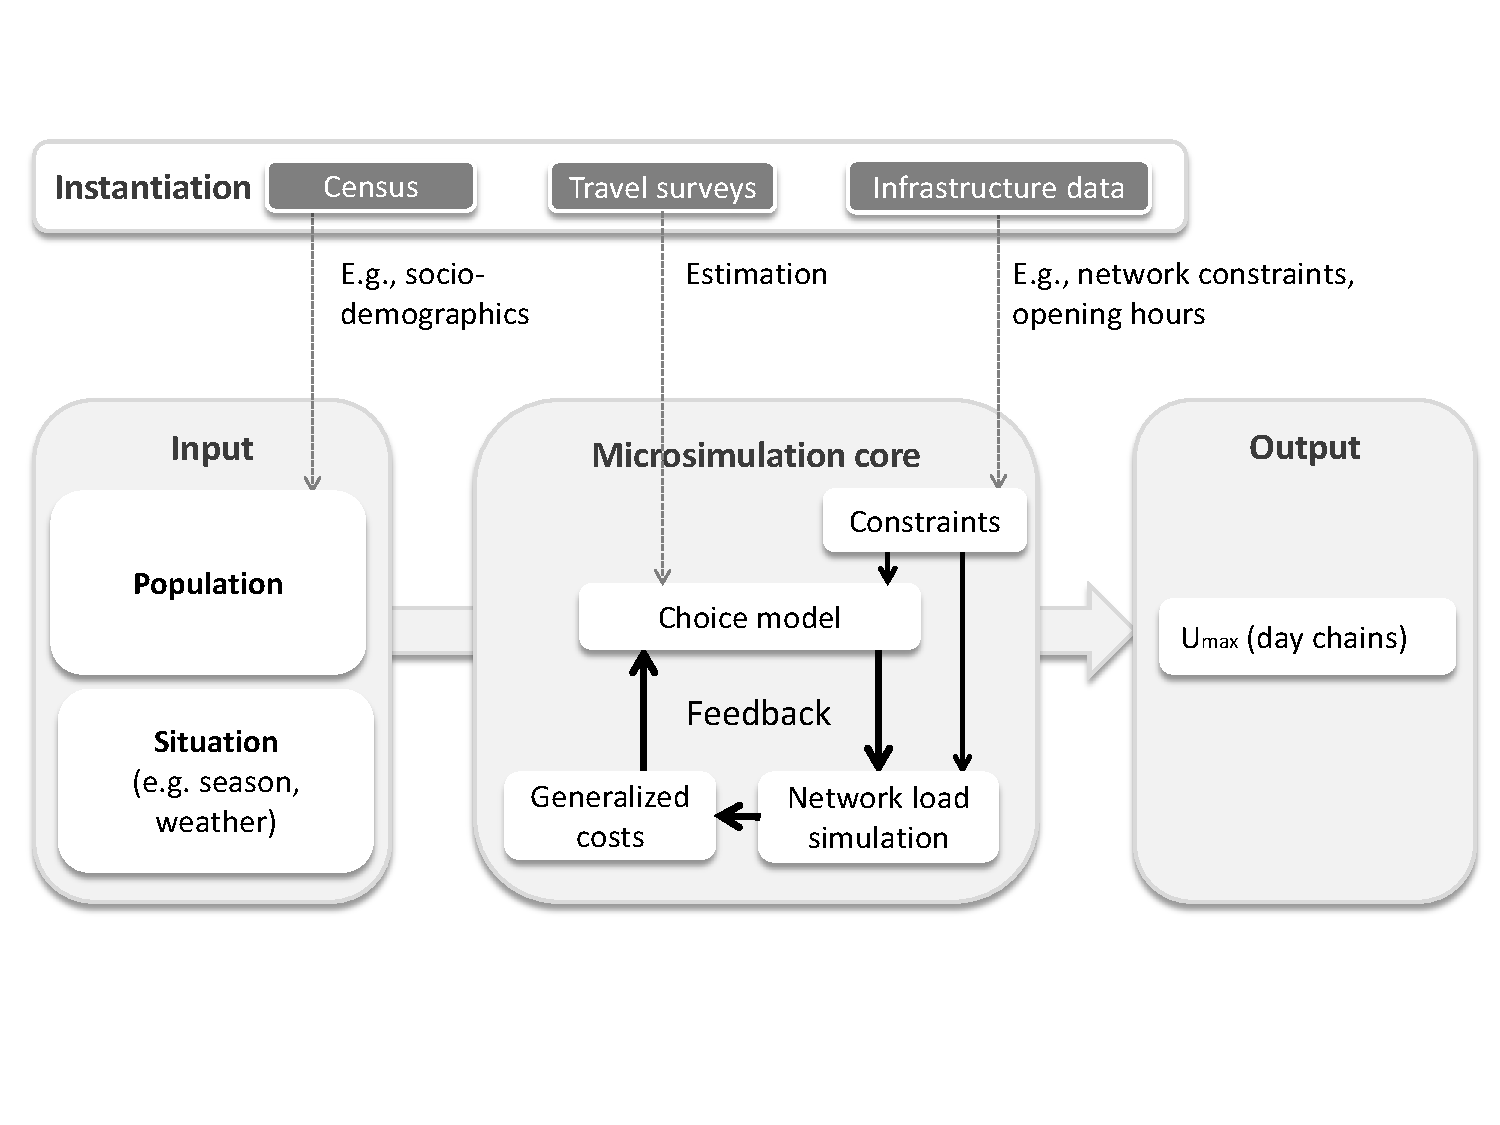
\includegraphics[width=0.99\textwidth, angle=0]{understanding/figures/maxUtf.pdf}}%
{}

% ----------
Note that this approach is really quite congruent with the SUE
approach: Every person has a collection of plans, which may be
interpreted as the choice set.  As in SUE, the choice set may be
generated while the iterations run or before the iterations start.
Every person selects between the plans, where one can attach to
every plan a score-based probability to be selected, 
in the end similar to Eq.~(\ref{stoch-equil}).
Clearly, a relevant research topic in this regards is to specify 
an evolutionary dynamic that can be shown to converge to choice sets
that are generated consistently with the requirements of discrete
choice theory; see Chapters~\ref{ch:discretechoice} and 
\note{REF research avenues}.
%%\todoKai{Der letzte Satz ersetzt einen anderen, der m.E.
%%an dieser Stelle keine neue Information mehr liefert. Gunnar}
%The main
%difference to SUE is once more that the choice ``fractions'' 
%%$q_{wp}$
%that appear per aggregate demand 
%%$q_w$ 
%are replaced by choice
%probabilities that appear per synthetic person.


%%\todoKai{Ein auskommentierter Absatz, der m.E. keine hierfuer relevante
%%  Information mehr liefert. Gunnar}
%No matter if one goes for a UE or a SUE,
%the equilibrium assignment of integer travelers is a
%combinatorial problem. 
%For a SUE, the conceptual and computational difficulties 
%that are associated with this type of problem can to some extent be
%circumvented by adopting a stochastic process perspective on the
%iterative simulation because repeated simulations of the same day 
%essentially allow to average out the discretization.
%This can be used to stabilize the simulation, and it also allows to 
%re-define convergence in terms of average conditions over many 
%iterations.

The following subsections give examples for the different elements of
this approach.


%%%%%%%%%%%%%%%%%%%%%%%%%%%%%%%%%%%%%%%%%%%%
%%%%%%%%%%%%%%%%%%%%%%%%%%%%%%%%%%%%%%%%%%%%
\subsubsection{Selection (choice)}
\label{sec:ag-based-assignment-selection}

%For choice, one can start with a logit model:
%\textbf{Selection/Choice:} 
A possible choice algorithm is the following: For persons with
unscored plans, select an unscored plan.  For all other persons,
select between existing plans with some SUE model, e.g.,\ a logit
model, i.e.,
\begin{equation}
P(i) = \frac{e^{\mu S_i}}{\sum_j e^{\mu S_j}} \
\label{eq:2}
\end{equation}
where $S_i$ is the score of plan $i$ and $\mu$ models the
travelers' ability to distinguish between plans of different
scores.
%
This is implemented in MATSim by \lstinline{SelectExpBeta}.

In practice, we have found that it is much better to not use
Eq.~(\ref{eq:2}) directly, but rather use a switching process that
\emph{converges} towards Eq.~(\ref{eq:2}).  
This can, for example, be
achieved by using a switching probability from $i$ to $j$ of
\begin{equation}
T(i \to j) = \gamma \,  e^{\beta ( S_j - S_i )/2} \ ,
\label{eq:3}
\end{equation}
%%\todoKai{Ich habe $\alpha$ durch $\gamma$ ersetzt, 
%%weil ersteres auch noch die learning rate beim score averaging ist. Gunnar}
where $i$ is the previous plan, $j$ is a randomly selected plan from
the same person, and $\gamma$ is a proportionality constant that needs
to be small enough so that the expression is never larger than one
(since it denotes a probability).  This works because the logit model
(\ref{eq:2})
%\begin{equation}
%p_i = \frac{1}{Z} \, e^{\beta S_i} \ ,
%\label{eq:4}
%\end{equation}
fulfills the detailed balance condition
\begin{equation}
P(i) \, T(i \to j) = P(j) \, T(j \to i) 
\label{eq:detailed-balance}
\end{equation}
for these $T(i \to j)$ \citep[e.g.,][]{ross-2006}.%
%%Since the process denoted by Eq.~(\ref{eq:3})
%%is ergodic, and the iterations eventually become Markovian, the logit
%%model Eq.~(\ref{eq:4}) denotes the unique equilibrium probability
%%distribution to that process.
\footnote{%
%
% Ich finde es nicht.  Aber die Logik müsste m.E. wie folgt sein:
%
% * Gegeben eine transition matrix T(i -> j).
%
% * Teste, ob es dafür Wahrscheinlichkeiten gibt, welche die detailed
%   balance condition erfüllen:
%     T(i -> j) p(i) = T(j -> i) p(j)
%
% * Falls ja, so ist das notwendigerweise eine stationäre Lösung (was
%   sich aus der Master-Gleichung ergibt).
%
% * Falls der Prozess auch noch ergodisch ist (Zustandsraum zerfällt
%   nicht in unverbundene Teile), dann sind diese W'en auch eindeutig.
%
% So ist es jetzt geschrieben.
%
% => Ich habe das unten zitierte Buch von Ross im Büro und schaue 
% da nochmal nach, wenn ich wieder im Buero bin. Gunnar
Assume that, after a number of iterations, there is no more
innovation, i.e., the choice set for every agent is fixed, and that
the scores are updated by MSA.
Upon convergence of the iterations, all agents draw their plans from
a fixed choice set based on constant score expectations, 
cf. (\ref{eq:sue-with-expectation}).
This means that all agents make their choices independently
(and that all interactions are captured in the scores).
The switching logic (\ref{eq:3}) then defines an ergodic Markovian process,
which converges to the unique steady state probabilities (\ref{eq:2}).
%%\todoKai{Neuer Versuch. Gunnar}
%Assume that, after a number of iterations, there is no more
%innovation, i.e., the choice set for every agent is fixed.
%%in the steady state.
%%
%This is now a Markovian process, which thus converges to steady
%state probabilities.
%%
%Since the process denoted by Eq.~(\ref{eq:3}) is ergodic, these
%probabilities are unique.
%%
%Assume that the scores, $\{S_i\}_i$, in the steady state eventually
%converge to some constant value (see Section \ref{sec:score-convergence}).
%%
%Since, in this situation, the logit probabilities, Eq.~(\ref{eq:2}),
%solve the detailed balance condition, Eq.~(\ref{eq:detailed-balance}),
%the logit probabilities \emph{are} the unique steady state
%probabilities.
%%%In this situation, the individual choice behavior fulfills
%%  detailed balance \citep{ross-2006} since the detailed balance equation
%%\[
%%p_i \, T(i \to j) = p_j \, T(j \to i) \ ,
%%\]
%%i.e.,
%%\[
%%p_i \, \alpha \,  e^{\beta ( S_j - S_i )/2} = p_j \, \alpha
%%\, e^{\beta ( S_i - S_j )/2} \ ,
%%\]
%%is solved by
%%\begin{equation}
%%\frac{p_i}{p_j} = e^{\beta ( S_i - S_j )} \ ,
%%\label{eq:1}
%%\end{equation}
%%which determinies the probabilities up to a multiplicative constant.
%
}
%
This is implemented in MATSim by \lstinline{ChangeExpBeta}.

The ``switching approach'' has additional advantages, including the
following:
\begin{itemize}

\item Eq.~(\ref{eq:3}) can be behaviorally interpreted as the
  probability of switching from plan $i$ to plan $j$.  Plausibly, this
  probability increases with the magnitude of the improvement.  

  For certain applications, one might desire a more involved approach,
  e.g., an \emph{expected} score of $j$ which then initiates the
  switch.

\item One could replace Eq.~(\ref{eq:3}) by a threshold-based
  dynamics, i.e.\ a switch to a better solution will only take place
  if the improvement is above a certain threshold.  The disadvantage
  is that one loses some of the mathematical interpretation, but the
  advantage is that it may be more consistent with some discussion in
  project appraisal where it is said that small improvements may not
  lead to a change in behavior.

%%\item If the difference between $S_j$ and $S_i$ is small, one can
%%  linearize Eq.~(\ref{eq:3}):
%%\begin{equation}
%%T(i \to j) \propto e^{\beta ( S_j - S_i )/2} 
%%%
%%\approx 1 + \frac{\beta}{2} \, (S_j - S_i) \ , 
%%\end{equation}
%%which means that a switching probability which is linear in the score
%%difference, often used in computer science/machine learning, is
%%mathematically related to the exponential switching probability
%%Eq.~(\ref{eq:2}), which, as explained, leads to the logit model.  

\end{itemize}

Although we have not done so systematically in past work, it is 
possible to include formulations such as path-size logit 
\citep{ben-akiva-1999} into the choice probabilities.

%\todoKai{????}  Overall, the approach has both a behavioral and a
%mathematical interpretation, and it is, in our view, most useful to
%move back and forth between the two.  For example, it is arguably
%quite plausible that travelers keep multiple options in mind, and
%that the network loading is stochastic because of stochasticity at
%\emph{all} levels, from driving to residential choice.  It is also
%quite plausible that the choice behavior \emph{does} depend directly
%on the experience from the previous day.  However, for mathematical
%reaons it may make sense to assume detailed balance; the question then
%becomes under which circumstances this is also behaviorally a
%reasonable assumption.  \todoKai{???}


%%%%%%%%%%%%%%%%%%%%%%%%%%%%%%%%%%%%%%%%%%%%
%%%%%%%%%%%%%%%%%%%%%%%%%%%%%%%%%%%%%%%%%%%%
\subsubsection{Score convergence}
\label{sec:score-convergence}

The assumption that the scores
%, $\{S_i\}_i$, 
eventually converge to
some constant value intuitively means that the scores cannot display
spontaneous reactive behavior to a certain iteration.  For example, it
might be possible that a particular iteration displays ``network
breakdown'' \citep{RieserNagel2008NetworkBreakdown}.  Converged scores
would not trigger a next-day reaction to that breakdown.  In practice,
this can be achieved by averaging the scores over many iterations,
which bears some similarity with ficticious play 
\citep{monderer-1996, garcia-2000}.
Once more, MSA is an option, with the same advantages and
disadvantages as discussed before.  An alternative is to us a small
\textbf{learning rate} $\alpha$ in
\begin{equation}
S_i^\text{new} = (1-\alpha) \, S_i^\text{old} + \alpha \, \tilde S_i \ ,
\end{equation}
where $S_i^{new}$ and $S_i^{old}$ are the agent's memorized scores for
option $i$, and $\tilde S_i$ is the most recent actual performance
with that option; see also Chapter~\ref{ch:discretechoice}.  
The issue, in the end, is the same as with the
stable-vs-unstable fixed points (cf.~Section~\ref{sec:agent-based-ue}):
If the system is well-behaved (corresponding to a stable fixed point),
it will converge benignly to constant scores and thus to the detailed
balance solution.  If the system is not well-behaved, one can still
force it to such a solution with MSA, but the meaning of this is less
clear.

As stated before, stochastic network loading makes no additional
conceptual difference, since there is already stochasticity caused by
the choice behavior.

%%\textbf{Stochastic network loading}, as stated earlier, simply means
%%that the scoring function now is stochastic.  Also with the SUE-like
%%approach, averaging over many draws is a theoretical option, but too
%%expensive in practice.  Fortunately, the approach with the learning
%%rate also works for stochastic network loading, although, all other
%%things unchanged, one needs a smaller learning rate $\alpha$.  That
%%is, different network loadings caused by different choices made by
%%other agents are treated the same way as different network loadings
%%caused by different random draws of the network loadings.

%%%%%%%%%%%%%%%%%%%%%%%%%%%%%%%%%%%%%%%%%%%%
%%%%%%%%%%%%%%%%%%%%%%%%%%%%%%%%%%%%%%%%%%%%
\subsubsection{Innovation (choice set generation)}

So far, this has left open the question concerning the choice set
\emph{generation}, i.e., the part that generates new plans or modifies
existing ones.  

One computationally simple technique that does not require a choice
set enumeration is to simulate randomly disturbed link costs and to
run best response based on these costs. This, however, can yield
unrealistic results if one does not get the correlation structure of
the noise right.

An alternative is to calculate separate best responses after every
network loading.  Since the process is stochastic, this will generate
different solutions from iteration to iteration.  An advantage is that
the correlations will be generated by the simulation -- and are, thus,
presumably realistic. Chapter~\ref{ch:discretechoice}
relates this to random utility modeling; see also Chapter~\note{REF research avenues}.
% A disadvantage is that there is currently
% little or no understanding how this relates to the noise
% specifications in random utility modeling.

Beyond that, there is really a myriad of different algorithms that
could be used here.  Besides the earlier-mentioned ``mutation''
\citep{BalmerRaneyEtAl2005act-times} or ``crossover''
\citep{CharyparNagel2005ga4acts,MeisterBalmerEtc2006planomatIatbr},
there are also many possibilities for constructive algorithms, such as
``agent-based'' construction
\citep{ZhuLevinsonZhang2008AgentBasedRouteChoice2}.  One attractive
option, clearly, is to use a regular activity-based demand generation
code \citep[e.g.,][]{BowmanEtc1999PortlandActs,MillerRoordaTASHA}
although our experience is that this may not be as simple as it seems
\citep{RieserNagelEtc2007early-berlin-trr} since in practice
activity-based models are often constructed with OD matrices in mind.  
A successful integration is described by 
\cite{ZiemkeNagelBhatIntegratingCemdapMatsimTransferability}.


%%Ramming \citep{Ben-AkivaRamming2005,RammingPhd} discusses route
%%generation algorithms that may be extended to daily plans. Zhu et al
%%discuss ``agent-based'' route choice  \citep{ZhuLevinsonEtAl2007Agent-basedRouteChoice}

%%%%However, alternative route generation algorithms are possible
%%%%\citep[e.g.][]{Ben-AkivaRamming2005,RammingPhd}.
%%\todoKai{``behavioral'' route gen somewhere else $\Rightarrow$ Passt
%%  meiner Meinung nach gut in der simulation section unter SUE. Gunnar}

%%\todoKai{maybe more, at least reference}


%%%%%%%%%%%%%%%%%%%%%%%%%%%%%%%%%%%%%%%%%%%%
%%%%%%%%%%%%%%%%%%%%%%%%%%%%%%%%%%%%%%%%%%%%
\subsubsection{Adjusting the ``improvement function'' from shortest
time to generalized utility functions}
\label{sec:adjust-impr-funct}

\def\perf{{\it perf}}

%%\todoKai{Ich habe dies jetzt noch zu einem Bestandteil der vorigen
%%Section gemacht, weil die utility function m.E. noch zu SUE gehoert.
%%Gunnar}

This chapter takes the inductive approach of arguing that one can make
the network assignment loop more general by including additional
choice dimensions beyond routing.  Clearly, for this to work the
computation of the scoring needs to take the effects of these
additional choice dimensions into account \citep[also
  see][]{Balmer2007phd}.  Given evolutionary game theory, it is quite
obvious how to do that: One has to extend the cost
function that is used for routing to a general scoring function for
complete daily plans.

%%\todoNextRevision{start with an example?}

That is, the performance of a daily plan needs to be scored.  An
established method to estimate scoring functions for different
alternatives is random utility theory \citep[e.g.][]{ben-akiva-1985},
which is why in the following, ``scoring'' will be replaced by
``utility''.  For a utility function for daily plans, the following
arguments may serve as starting points:
\begin{itemize}

\item A heuristic approach, consistent with wide-spread assumptions
  about travel behavior, is to give positive rewards to performing an
  activity and negative rewards to travelling.

\item For the activities, one should select functions where the
  marginal reward of doing an activity decreases over time.
  %%\todoNextRevision{read Feil/Joh!}

\item Without additional effects, such as opening times or
  time-varying congestion, the marginal utilities of all performed
  activities should be the same.  

\end{itemize}
MATSim has, in the past years, gained some experience with the approach 
described in Chapter~\ref{ch:scoring} and with more theory in 
Chapter~\ref{ch:economicEval}; this then closes the loop.  


%%%%%%%%%%%%%%%%%%%%%%%%%%%%%%%%%%%%%%%%%%%%
%%%%%%%%%%%%%%%%%%%%%%%%%%%%%%%%%%%%%%%%%%%%
\section{Conclusion}
\label{sec:agentbased-dta-conclusion}

% This paper investigates how behavioral considerations can be
% integrated into the modeling of network dynamics.  
Starting from
regular route assignment, this chapter points out that one can extend the
iterative solution procedure of static or dynamic traffic assignment
to include additional behavioral dimensions such as time adaptation,
mode choice or secondary activity location choice.  This is somewhat
similar to the so-called supernetworks approach, but argues from the
viewpoint of the iterative solution procedure rather than from the
viewpoint of the problem definition.

In order to address the combinatorial explosion of the commodities
caused by the expansion of the choice dimensions, it is suggested to
move to individual particles.  This allows an interpretation of the
solution procedure as behavioral day-to-day learning, but maintains a
connection to the SUE definition by interpreting the synthetic
travellers' behavior as random draws from individual choice sets.  
% In
% that latter interpretation, the iterative solution procedure becomes a
% Monte Carlo simulation that samples from the population's choice
% distribution.

A major part of this chapter discusses simulation/computer implementation issues.
From the definition given above, progress can be made by using methods
from machine learning and co-evolutionary search algorithms.  
%
The SUE problem of random selection between different alternatives can
be cast as a so-called population-based optimization algorithm where
every synthetic traveler randomly selects between the different
members of the population of possible solutions.
%
At the same time, the \emph{population of the travelers} co-evolves
towards a stationary distribution of choices.

Overall, this chapter has worked out the structural similarity between the 
``classical" DTA problem and the more recent agent-based assignment problem.
The presentation has focused on the algorithmic issue of how to find solutions 
of these problems. This is complemented by the subsequent Chapters~\ref{ch:montecarlo} to \ref{ch:kinematicwaves}, 
which mostly discuss modeling (descriptive) aspects of MATSim.

\gunnar{Hier w\"urde sich vielleicht noch ein kleiner (eher technischer) Appendix 
zum Thema ``running MATSim as a standard DTA'' anbieten.}

% %%\todoKai{Mit diesem Schluss-Paragraphen habe ich Probleme.  Vorschlaege?
% %%  weglassen?  Kai $\Rightarrow$ Hab's mal versucht. Gunnar}
% Overall, it has been clear for some time now that it is possible to
% simulate large transportation systems microscopically, including many
% learning iterations with choice dimensions beyond route choice, and
% this paper describes some of the necessary methods and techniques.
% %
% Future research will have to fill the gap between the computationally
% efficient yet behaviorally simplified approaches that have by now been
% demonstrated to be applicable to large real-world scenarios and the
% far more sophisticated yet less operational behavioral models proposed 
% in the travel demand literature.
% %%
% %An arguably newer development, also described in this paper, is how
% %such micro-simulations can be interpreted as Monte Carlo draws from
% %some underlying distributions that are related to the SUE definition. 
% %%
% %This opens the door to a solid mathematical foundation of the
% %approach.

%%%%%%%%%%%%%%%%%%%%%%%%%%%%%%%%%%%%%%%%%%%%
%%%%%%%%%%%%%%%%%%%%%%%%%%%%%%%%%%%%%%%%%%%%
%% \section{Acknowledgements}

%% This paper derives much from the MATSim project, which is a
%% collaboration between many people and institutions.  For the issues
%% investigated in this paper, we benefited from discussions with
%% %
%% M.~Bierlaire,
%% A.~Borning, % uw cs search project
%% D.~Fox, % uw cs search project
%% P.~Henry, % uw cs search project
%% D.~Layton, % uw cs search project
%% F.~Marchal, 
%% F.~Martinez,
%% %
%% and P.~Waddell.

%%%%%%%%%%%%%%%%%%%%%%%%%%%%%%%%%%%%%%%%%%%%
%%%%%%%%%%%%%%%%%%%%%%%%%%%%%%%%%%%%%%%%%%%%

% Local Variables:
% mode: latex
% mode: reftex
% mode: visual-line
% TeX-master: "../main"
% comment-padding: 1
% fill-column: 9999
% End: 
